\documentclass[]{article}

% Imported Packages
%------------------------------------------------------------------------------
\usepackage{amssymb}
\usepackage{amstext}
\usepackage{amsthm}
\usepackage{amsmath}
\usepackage{enumerate}
\usepackage{fancyhdr}
\usepackage[margin=1in]{geometry}
\usepackage{graphicx}
\usepackage[inkscapeformat=png]{svg}
\usepackage{float}
%\usepackage{extarrows}
\usepackage{booktabs}
%\usepackage{setspace}
%------------------------------------------------------------------------------

% Header and Footer
%------------------------------------------------------------------------------
\pagestyle{plain}  
\renewcommand\headrulewidth{0.4pt}                                      
\renewcommand\footrulewidth{0.4pt}                                    
%------------------------------------------------------------------------------

% Title Details
%------------------------------------------------------------------------------
\title{Deliverable \#2 Template}
\author{SE 3A04: Software Design II -- Large System Design}
\date{}                               
%------------------------------------------------------------------------------

% Document
%------------------------------------------------------------------------------
\begin{document}

\setlength{\parindent}{0pt}

\maketitle	
\noindent{\bf Tutorial Number:} T03\\
{\bf Group Number:} G07 \\
{\bf Group Members:} 
\begin{itemize}
	\item Farid Bastoros 
	\item Neha Bhatla
	\item Omar Alam
	\item Luka Mahrt-Smith
	\item Aidan Lao
\end{itemize}

\section*{IMPORTANT NOTES}
\begin{itemize}
	%	\item You do \underline{NOT} need to provide a text explanation of each diagram; the diagram should speak for itself
	\item Please document any non-standard notations that you may have used
	\begin{itemize}
		\item \emph{Rule of Thumb}: if you feel there is any doubt surrounding the meaning of your notations, document them
	\end{itemize}
	\item Some diagrams may be difficult to fit into one page
	\begin{itemize}
		\item Ensure that the text is readable when printed, or when viewed at 100\% on a regular laptop-sized screen.
		\item If you need to break a diagram onto multiple pages, please adopt a system of doing so and thoroughly explain how it can be reconnected from one page to the next; if you are unsure about this, please ask about it
	\end{itemize}
	\item Please submit the latest version of Deliverable 1 with Deliverable 2
	\begin{itemize}
		\item Indicate any changes you made.
	\end{itemize}
	\item If you do \underline{NOT} have a Division of Labour sheet, your deliverable will \underline{NOT} be marked
\end{itemize}

\newpage
\section{Introduction}
\label{sec:introduction}
% Begin Section

% This section should provide an brief overview of the entire document.

\subsection{Purpose}
\label{sub:purpose}
% Begin SubSection
This document provides a high-level overview of the Shroomify system architecture, outlining the core design principles, subsystems, and the rationale behind architectural choices. It is intended for internal stakeholders involved in the development of Shroomify, including software engineers, project managers, investors, domain experts, and system architects. Prior technical knowledge is beneficial but not required for understanding this document. \\
Please ensure that Shroomify Deliverable 1 is reviewed before Deliverable 2, as it provides essential context. Additionally, having technical knowledge may help in better understanding the contents of this document.
% End SubSection

\subsection{System Description}
\label{sub:system_description}
% Begin SubSection
The Shroomify system follows a Model-View-Controller (MVC) architecture, separating data management, business logic, and user interactions. This type of architecture has Model components, View components and Controller components which increase its scalability and  maintainability, allowing each component to be tested and updated independently.\\

\noindent Additionally, Shroomify integrates Blackboard architecture and Repository architecture for  different subsystems based on their functionality. The repository architecture was used for subsystems that require efficient data storage and retrieval, allowing for concurrent access to shared data repositories. The Blackboard architecture was used for subsystems that need to combine different pieces of information to reach a final result, making it useful for tasks like decision-making and identification.

% End SubSection

\subsection{Overview}
\label{sub:overview}
% Begin SubSection
This is Deliverable 2 of the Shroomify project and provides a general description of the system architecture. It considers the requirements, use cases, and design decisions outlined in Deliverable 1. Section 2 has an Analysis Class Diagram that represents the major classes and how they relate to each other from our requirements analysis. This diagram establishes the foundation for the organization of the system internally and ensures that design is high in cohesion and low in coupling among its components. Section 3 presents a description of the Architectural Design of Shroomify. In this section, we define the chosen architectural pattern and discuss specific design decisions. Section 4 focused on Class Responsibility Collaboration (CRC) Cards. These cards capture the responsibilities and communications of each class within the system, detailing exactly how the individual components interact to satisfy the demands of the system.\\
Collectively, these sections provide a solid foundation for understanding the structure and functionality of the Shroomify app.
% End SubSection

% End Section
\clearpage
\section{Analysis Class Diagram}
\label{sec:analysis_class_diagram}
% Begin Section
% This section should provide an analysis class diagram for your application.
\begin{figure}[h]
    \centering
    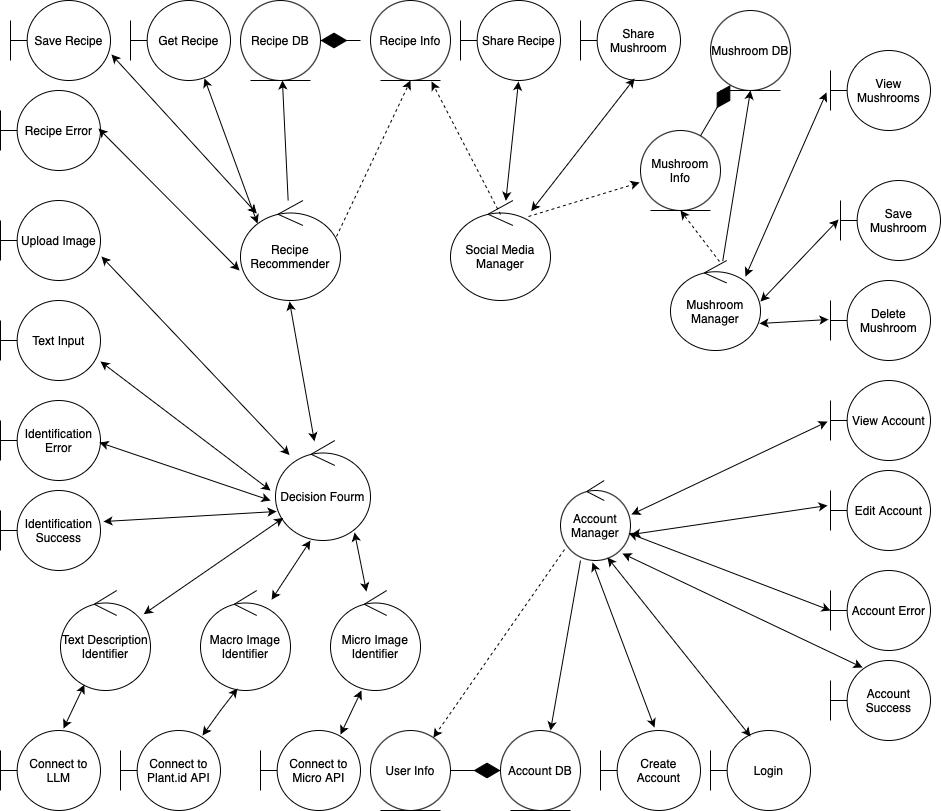
\includegraphics[width=1\textwidth]{AnalysisClassDiagram.png}
    \caption{Analysis Class Diagram}
    \label{fig:sample}
\end{figure}
% End Section

\clearpage
\section{Architectural Design}
\label{sec:architectural_design}

\subsection{System Architecture}
\label{sub:system_architecture}

% End SubSection

Shroomify uses the \textbf{Model-View-Controller (MVC)} architectural pattern 
as the main architecture of the system. Within the MVC pattern, the system is 
divided into three main component types: the \textbf{Model} components, the \textbf{View} components, and 
the \textbf{Controller} components. The \textbf{Model} components are responsible for managing 
data storage in the system. The \textbf{View} components are responsible 
for displaying the various user interface pages. The \textbf{Controller} components 
are responsible for handling user input and updating the models and views accordingly. 
The MVC pattern was chosen for Shroomify because it provides a clear 
separation of concerns between the different components of the system, 
making it easier to maintain and extend the system in the future. The MVC 
pattern also allows for the system to be easily tested, as each component 
can be tested independently of the others.

\vspace{5pt}
For each subsystem, we have identified different architectures that will be used:
\begin{table}[H]
	\centering
	\begin{tabular}{cp{7cm}p{4cm}}
		\toprule
		Subsystem & Tasks & Architecture \\
		\midrule
		Decision Forum & Take partial solutions from expert agents and produce final identification solution. & Blackboard Architecture \\
		Mushroom Management & Store and modify information related to mushrooms identified by the user in a database. & Repository Architecture \\
		Account Management & Manage account registration and modification.  & Repository Architecture \\
		Social Media Management & Handle information sharing with external social media platforms. & Model-View-Controller Architecture\\
		Recipe Recommendation & Recommend recipes to user based on identified mushrooms. & Repository Architecture \\
		\bottomrule
	\end{tabular}
	\caption{Subsystem Architectures}
\end{table}

\subsubsection{Decision Forum Architecture}

The blackboard architecture was chosen for the Decision Forum subsystem because it is well-suited
to combine partial solutions from different expert software agents such as the \textbf{Text Description Identifier},
\textbf{Macro Image Identifier}, and \textbf{Micro Image Identifier}. The blackboard architecture
allows these agents to work independently and asynchronously, and then combine their partial 
solutions to produce a final identification solution. This architecture is well-suited to the 
Decision Forum subsystem because it allows for the integration of multiple expert agents with 
different areas of expertise, and provides a flexible and extensible framework for combining 
their solutions. It also allows for us to easily modify each agent independently without affecting
the overall system and also add more agents if needed in the future without any modification of pre-existing
code. This architecture lets us apply the open-closed principle well which will help us with maintainability
in the future. Another architecture that was considered for this subsystem was the Model-View-Controller
architecture, but it was not chosen because the Decision Forum subsystem is not primarily focused on user
interaction and does not require a user interface. MVC also does not provide a clear way to combine
the partial solutions from different expert agents.

\subsubsection{Mushroom Management Architecture}

The repository architecture was chosen for the Mushroom Management subsystem because it is well-suited
for the simple data storage and retrieval tasks required by this subsystem. The repository architecture
provides a data store that can be accessed by software agents in different ways.

\subsubsection{Account Management Architecture}

The repository architecture was chosen for the Account Management subsystem for the same reasons 
as the Mushroom Management subsystem. The Account Management subsystem also requires simple data
storage and retrieval tasks, and the repository architecture provides a flexible data store 
system.

\subsubsection{Social Media Management Architecture}

The Model-View-Controller architecture was chosen for the Social Media Management subsystem since 
a user interaction will be required to share information with external social media platforms. This entails
having a user interface to interact with the system (View), an agent to handle user input (Controller), and 
a data store to manage the retrieve and store the information being shared (Model). The pipe and filter
architecture was considered because of the nature of the subsystem sending streams of information to 
external platforms, and it may be contained within the controller of the architecture but is not well-suited
to be the main architecture for the subsystem.

\subsubsection{Recipe Recommendation Architecture}

The repository architecture was chosen for the Recipe Recommendation subsystem since the Recommendation
system is intended to be a simple search and compare algorithm from a database. The architecture provides
a data store (database) which can be efficiently searched for recipes based on the identified mushrooms.
The blackboard architecture was considered for this subsystem because it could potentially combine multiple 
recommendation algorithms to produce a final recommendation. However, the complexity of the recommendation
system is not high enough to warrant the use of the blackboard architecture.

\newpage
The following diagrams show the structural architecture of the system, illustrating the 
relationships between different controllers, databases and views.

\begin{figure}[H]
	\centering
	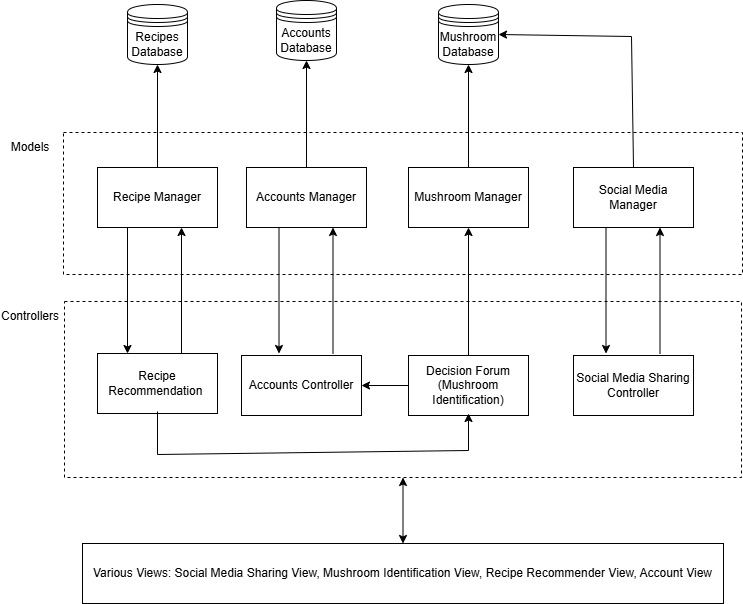
\includegraphics[width=1\textwidth]{sysarch.png}
	\caption{Model-View-Controller Architecture}
	\label{fig:sys-arch}
\end{figure}

\begin{figure}[H]
	\centering
	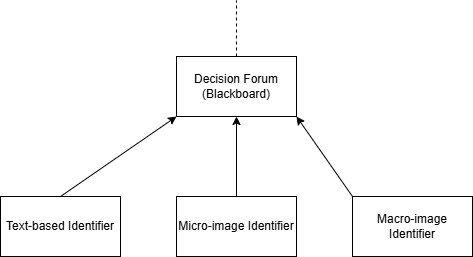
\includegraphics[width=0.6\textwidth]{blackboard-df.png}
	\caption{Blackboard Architecture for Decision Forum}
	\label{fig:blackboard}
\end{figure}


% \paragraph{Purpose}
\subsection{Subsystems}
Our system is divided into five main subsystems: \textbf{Decision Forum, Mushroom Management, Account Management, Social Media Management, and Recipe Recommendation}. These subsystems interact to provide users with a seamless experience in identifying mushrooms, managing their findings, and sharing information.

\subsubsection{Decision Forum}
The \textbf{Decision Forum} subsystem is responsible for identifying mushrooms. It contains the \textbf{machine learning algorithm} that classifies mushrooms based on user-provided descriptions and \textbf{computer vision technology} that analyzes images to determine species. If the identification confidence is low, users can also post images and descriptions to receive verification from the community.
 
\paragraph{Purpose}
Automates mushroom identification using AI and provides a space for community-based verification.
 
\paragraph{Relationship to Other Subsystems}
\begin{itemize}
    \item Works with \textbf{Mushroom Management} to store confirmed identifications.
    \item Interfaces with \textbf{Account Management} to associate identifications with users.
    \item Can interact with \textbf{Social Media Management} for users to share identification discussions.
\end{itemize}
 
\subsubsection{Mushroom Management}
The \textbf{Mushroom Management} subsystem serves as a \textbf{personal dictionary} of previously identified mushrooms. It allows users to view mushrooms they’ve found in the past, track their quantity, and access relevant information, including images and descriptions.
 
\paragraph{Purpose}
Stores and displays user-identified mushrooms but does \textbf{not} perform identification itself.
 
\paragraph{Relationship to Other Subsystems}
\begin{itemize}
    \item Retrieves identification results from \textbf{Decision Forum} and saves them.
    \item Integrates with \textbf{Account Management} to store mushroom data within user profiles.
    \item Interfaces with \textbf{Recipe Recommendation} to provide relevant recipes for identified mushrooms.
\end{itemize}
 
\subsubsection{Account Management}
The \textbf{Account Management} subsystem handles user authentication, profile settings, and data storage. It maintains a personalized record of identified mushrooms and user activity.
 
\paragraph{Purpose}
Manages user profiles and ensures that each user’s mushroom data is securely stored.
 
\paragraph{Relationship to Other Subsystems}
\begin{itemize}
    \item Stores user-identified mushrooms from \textbf{Mushroom Management}.
    \item Maintains user participation history in \textbf{Decision Forum}.
    \item Interfaces with \textbf{Social Media Management} to track and share posts.
\end{itemize}
 
\subsubsection{Social Media Management}
The \textbf{Social Media Management} subsystem allows users to share their mushroom identifications, forum discussions, and recipes on external platforms such as Facebook, Instagram, and Twitter.
 
\paragraph{Purpose}
Enhances community engagement by enabling content sharing.
 
\paragraph{Relationship to Other Subsystems}
\begin{itemize}
    \item Works with \textbf{Account Management} to post from user profiles.
    \item Allows users to share discoveries from \textbf{Mushroom Management} and \textbf{Decision Forum}.
    \item Enables recipe-sharing from \textbf{Recipe Recommendation}.
\end{itemize}
 
\subsubsection{Recipe Recommendation}
The \textbf{Recipe Recommendation} subsystem suggests safe and relevant recipes based on identified mushrooms. It retrieves information from a database and presents culinary suggestions to users.
 
\paragraph{Purpose}
Provides users with potential culinary uses for their identified mushrooms.
 
\paragraph{Relationship to Other Subsystems}
\begin{itemize}
    \item Works with \textbf{Mushroom Management} to access user-identified mushrooms.
    \item Allows users to share recipes through \textbf{Social Media Management}.
\end{itemize}
 % End SubSection

% End Section
\clearpage	
\section{Class Responsibility Collaboration (CRC) Cards}
\label{sec:class_responsibility_collaboration_crc_cards}
% Begin Section
This section should contain all of your CRC cards.

\begin{itemize}
	\item Provide a CRC Card for each identified class
	% \item Please use the format outlined in tutorial, i.e., 
	\begin{table}[ht]
		\centering
		\begin{tabular}{|p{6cm}|p{6cm}|}
		\hline 
		\multicolumn{2}{|l|}{\textbf{Class Name: Recipe Recommender (Controller)}} \\
		\hline
		\textbf{Responsibility:} & \textbf{Collaborators:} \\
		\hline
		Knows Get Recipe & Get Recipe\\
		Knows Save Recipe & Save Recipe\\
		Knows Recipe Error & Recipe Error\\
		Knows Recipe DB & Recipe DB\\
		Knows Decision Fourm & Decision Fourm\\
		Knows Recipe Info & Recipe Info\\
		\vspace{1in} & \\
		\hline
		\end{tabular}
	\end{table}
	\begin{table}[ht]
		\centering
		\begin{tabular}{|p{6cm}|p{6cm}|}
		\hline 
		\multicolumn{2}{|l|}{\textbf{Class Name: Recipe Info (Entity)}} \\
		\hline
		\textbf{Responsibility:} & \textbf{Collaborators:} \\
		\hline
		Knows Recipe Recommender & Recipe Recommender \\
		Knows Recipe DB & Recipe DB \\
            Knows Social Media Manager & Social Media Manager \\
		\vspace{1in} & \\
		\hline
		\end{tabular}
	\end{table}
	\begin{table}[ht]
		\centering
		\begin{tabular}{|p{6cm}|p{6cm}|}
		\hline 
		\multicolumn{2}{|l|}{\textbf{Class Name: Recipe DB (Entity)}} \\
		\hline
		\textbf{Responsibility:} & \textbf{Collaborators:} \\
		\hline
		Knows Recipe Recommender & Recipe Recommender \\
		Knows Recipe Info & Recipe Info \\
		\vspace{1in} & \\
		\hline
		\end{tabular}
	\end{table}
	\begin{table}[ht]
		\centering
		\begin{tabular}{|p{6cm}|p{6cm}|}
		\hline 
		\multicolumn{2}{|l|}{\textbf{Class Name: Get Recipe (Boundary)}} \\
		\hline
		\textbf{Responsibility:} & \textbf{Collaborators:} \\
		\hline
		Knows Recipe Recommender & Recipe Recommender \\
		Handles click event of “Get Recipe” button & \\  
		\vspace{1in} & \\
		\hline
		\end{tabular}
	\end{table}
	\begin{table}[ht]
		\centering
		\begin{tabular}{|p{6cm}|p{6cm}|}
		\hline 
		\multicolumn{2}{|l|}{\textbf{Class Name: Save Recipe (Boundary)}} \\
		\hline
		\textbf{Responsibility:} & \textbf{Collaborators:} \\
		\hline
		Knows Recipe Recommender & Recipe Recommender \\
		Handles click event of “Save Recipe” button & \\
		\vspace{1in} & \\
		\hline
		\end{tabular}
	\end{table}
	\begin{table}[ht]
		\centering
		\begin{tabular}{|p{6cm}|p{6cm}|}
		\hline 
		\multicolumn{2}{|l|}{\textbf{Class Name: Recipe Error (Boundary)}} \\
		\hline
		\textbf{Responsibility:} & \textbf{Collaborators:} \\
		\hline
		Knows Recipe Recommender & Recipe Recommender \\
		Handles Get Recipe error events & \\
		Handles Save Recipe error events & \\
		\vspace{1in} & \\
		\hline
		\end{tabular}
	\end{table}
	\begin{table}[ht]
		\centering
		\begin{tabular}{|p{6cm}|p{6cm}|}
		\hline 
		\multicolumn{2}{|l|}{\textbf{Class Name: Decision Fourm (Controller)}} \\
		\hline
		\textbf{Responsibility:} & \textbf{Collaborators:} \\
		\hline
		Knows Upload Image & Upload Image \\
		Knows Text Input & Text Input \\
		Knows Identification Error & Identification Error \\
		Knows Identification Success & Identification Success \\
		Knows Text Description Identifier &  Text Description Identifier \\
		Knows Macro Image Identifier & Macro Image Identifier \\
		Knows Micro Image Identifier & Micro Image Identifier \\
		Knows Recipe Recommender & Recipe Recommender \\

		\vspace{1in} & \\
		\hline
		\end{tabular}
	\end{table}
	\begin{table}[ht]
		\centering
		\begin{tabular}{|p{6cm}|p{6cm}|}
		\hline 
		\multicolumn{2}{|l|}{\textbf{Class Name: Text Description Identifier (Controller)}} \\
		\hline
		\textbf{Responsibility:} & \textbf{Collaborators:} \\
		\hline
		Knows Connect to LLM & Connect to LLM \\
		Knows Decision Fourm & Decision Fourm \\ 
		\vspace{1in} & \\
		\hline
		\end{tabular}
	\end{table}
	\begin{table}[ht]
		\centering
		\begin{tabular}{|p{6cm}|p{6cm}|}
		\hline 
		\multicolumn{2}{|l|}{\textbf{Class Name: Macro Image Identifier (Controller)}} \\
		\hline
		\textbf{Responsibility:} & \textbf{Collaborators:} \\
		\hline
		Knows Connect to plant.id API & Connect to plant.id API \\
		Knows Decision Fourm & Decision Fourm \\ 
		\vspace{1in} & \\
		\hline
		\end{tabular}
	\end{table}
	\begin{table}[ht]
		\centering
		\begin{tabular}{|p{6cm}|p{6cm}|}
		\hline 
		\multicolumn{2}{|l|}{\textbf{Class Name: Micro Image Identifier (Controller)}} \\
		\hline
		\textbf{Responsibility:} & \textbf{Collaborators:} \\
		\hline
		Knows Connect to Micro API & Connect to Micro API \\
		Knows Decision Fourm & Decision Fourm \\ 
		\vspace{1in} & \\
		\hline
		\end{tabular}
	\end{table}
	\begin{table}[ht]
		\centering
		\begin{tabular}{|p{6cm}|p{6cm}|}
		\hline 
		\multicolumn{2}{|l|}{\textbf{Class Name: Upload Image (Boundary)}} \\
		\hline
		\textbf{Responsibility:} & \textbf{Collaborators:} \\
		\hline
		Knows Decision Fourm & Decision Fourm \\
		Handles click event of “Upload Image” button & \\
		\vspace{1in} & \\
		\hline
		\end{tabular}
	\end{table}
	\begin{table}[ht]
		\centering
		\begin{tabular}{|p{6cm}|p{6cm}|}
		\hline 
		\multicolumn{2}{|l|}{\textbf{Class Name: Text Input (Boundary)}} \\
		\hline
		\textbf{Responsibility:} & \textbf{Collaborators:} \\
		\hline
		Knows Decision Fourm & Decision Fourm \\
		Handles click event of “Text Input” button & \\
		\vspace{1in} & \\
		\hline
		\end{tabular}
	\end{table}
	\begin{table}[ht]
		\centering
		\begin{tabular}{|p{6cm}|p{6cm}|}
		\hline 
		\multicolumn{2}{|l|}{\textbf{Class Name: Identification Error (Boundary)}} \\
		\hline
		\textbf{Responsibility:} & \textbf{Collaborators:} \\
		\hline
		Knows Decision Fourm & Decision Fourm \\
		Handles Upload Image error events & \\
		Handles Text Input error events & \\
		\vspace{1in} & \\
		\hline
		\end{tabular}
	\end{table}
	\begin{table}[ht]
		\centering
		\begin{tabular}{|p{6cm}|p{6cm}|}
		\hline 
		\multicolumn{2}{|l|}{\textbf{Class Name: Identification Success (Boundary)}} \\
		\hline
		\textbf{Responsibility:} & \textbf{Collaborators:} \\
		\hline
		Knows Decision Fourm & Decision Fourm \\
		Handles Successful events of Upload Image & \\
		Handles Successful events of Text Input & \\
		\vspace{1in} & \\
		\hline
		\end{tabular}
	\end{table}
	\begin{table}[ht]
		\centering
		\begin{tabular}{|p{6cm}|p{6cm}|}
		\hline 
		\multicolumn{2}{|l|}{\textbf{Class Name: Connect to LLM  (Boundary)}} \\
		\hline
		\textbf{Responsibility:} & \textbf{Collaborators:} \\
		\hline
		Knows Text Description Identifier & Text Description Identifier \\
		Handles click event of “Identify Mushroom” button & \\
		\vspace{1in} & \\
		\hline
		\end{tabular}
	\end{table}
	\begin{table}[ht]
		\centering
		\begin{tabular}{|p{6cm}|p{6cm}|}
		\hline 
		\multicolumn{2}{|l|}{\textbf{Class Name: Connect to Plant.id API (Boundary)}} \\
		\hline
		\textbf{Responsibility:} & \textbf{Collaborators:} \\
		\hline
		Knows Text Description Identifier & Text Description Identifier \\
		Handles click event of “Identify Mushroom” button & \\
		\vspace{1in} & \\
		\hline
		\end{tabular}
	\end{table}
	\begin{table}[ht]
		\centering
		\begin{tabular}{|p{6cm}|p{6cm}|}
		\hline 
		\multicolumn{2}{|l|}{\textbf{Class Name: Connect to  Micro API (Boundary)}} \\
		\hline
		\textbf{Responsibility:} & \textbf{Collaborators:} \\
		\hline
		Knows Text Description Identifier & Text Description Identifier \\
		Handles click event of “Identify Mushroom” button & \\
		\vspace{1in} & \\
		\hline
		\end{tabular}
	\end{table}

	\begin{table}[ht]
		\centering
		\begin{tabular}{|p{6cm}|p{6cm}|}
		\hline 
		\multicolumn{2}{|l|}{\textbf{Class Name: Account Manager (Controller)}} \\
		\hline
		\textbf{Responsibility:} & \textbf{Collaborators:} \\
		\hline
            Knows Account DB & Account DB\\
		Knows User Info & User Info\\
		Knows Create Account & Create Account\\
            Knows Edit Account & Edit Account\\
		Knows View Account & View Account\\
		Knows Login & Login\\
            Knows Account Success & Account Success\\
            Knows Account Error & Account Error\\

		\vspace{1in} & \\
		\hline
		\end{tabular}
	\end{table}

        \begin{table}[ht]
		\centering
		\begin{tabular}{|p{6cm}|p{6cm}|}
		\hline 
		\multicolumn{2}{|l|}{\textbf{Class Name: Account DB  (Entity)}} \\
		\hline
		\textbf{Responsibility:} & \textbf{Collaborators:} \\
		\hline
		Knows Account Manager & Account Manager\\
		Knows User Info & User Info\\
		\vspace{1in} & \\
		\hline
		\end{tabular}
	\end{table}

        \begin{table}[ht]
		\centering
		\begin{tabular}{|p{6cm}|p{6cm}|}
		\hline 
		\multicolumn{2}{|l|}{\textbf{Class Name: User Info (Entity)}} \\
		\hline
		\textbf{Responsibility:} & \textbf{Collaborators:} \\
		\hline
		Knows Account Manager & Account Manager\\
            Knows Account DB & Account DB\\
		\vspace{1in} & \\
		\hline
		\end{tabular}
	\end{table}

    \begin{table}[ht]
		\centering
		\begin{tabular}{|p{6cm}|p{6cm}|}
		\hline 
		\multicolumn{2}{|l|}{\textbf{Class Name: Create Account (Boundary)}} \\
		\hline
		\textbf{Responsibility:} & \textbf{Collaborators:} \\
		\hline
		Knows Account Manager & Account Manager\\
            Handle user interactions for creating an account &\\
		\vspace{1in} & \\
		\hline
		\end{tabular}
	\end{table}

        \begin{table}[ht]
		\centering
		\begin{tabular}{|p{6cm}|p{6cm}|}
		\hline 
		\multicolumn{2}{|l|}{\textbf{Class Name: Edit Account (Boundary)}} \\
		\hline
		\textbf{Responsibility:} & \textbf{Collaborators:} \\
		\hline
		Knows Account Manager & Account Manager\\
            Handles click-event of "Edit Account" button &\\
		\vspace{1in} & \\
		\hline
		\end{tabular}
	\end{table}

        \begin{table}[ht]
		\centering
		\begin{tabular}{|p{6cm}|p{6cm}|}
		\hline 
		\multicolumn{2}{|l|}{\textbf{Class Name: View Account (Boundary)}} \\
		\hline
		\textbf{Responsibility:} & \textbf{Collaborators:} \\
		\hline
		Knows Account Manager & Account Manager\\
            Handles click-event of "View Account" button &\\
		\vspace{1in} & \\
		\hline
		\end{tabular}
	\end{table}

        \begin{table}[ht]
		\centering
		\begin{tabular}{|p{6cm}|p{6cm}|}
		\hline 
		\multicolumn{2}{|l|}{\textbf{Class Name: Login (Boundary)}} \\
		\hline
		\textbf{Responsibility:} & \textbf{Collaborators:} \\
		\hline
		Knows Account Manager & Account Manager\\
            Handles click-event of "Login" button &\\
		\vspace{1in} & \\
		\hline
		\end{tabular}
	\end{table}

        \begin{table}[ht]
		\centering
		\begin{tabular}{|p{6cm}|p{6cm}|}
		\hline 
		\multicolumn{2}{|l|}{\textbf{Class Name: Account Success (Boundary)}} \\
		\hline
		\textbf{Responsibility:} & \textbf{Collaborators:} \\
		\hline
		Knows Account Manager & Account Manager\\
            Handles successful events for account creation/editing & \\
		\vspace{1in} & \\
		\hline
		\end{tabular}
	\end{table}

        \begin{table}[ht]
		\centering
		\begin{tabular}{|p{6cm}|p{6cm}|}
		\hline 
		\multicolumn{2}{|l|}{\textbf{Class Name: Account Error (Boundary)}} \\
		\hline
		\textbf{Responsibility:} & \textbf{Collaborators:} \\
		\hline
		Knows Account Manager & Account Manager\\
            Handles Login error events &  \\
            Handles Edit Account error events & \\
            Handles View Account error events &  \\
		\vspace{1in} & \\
		\hline
		\end{tabular}
	\end{table}

     \begin{table}[ht]
		\centering
		\begin{tabular}{|p{6cm}|p{6cm}|}
		\hline 
		\multicolumn{2}{|l|}{\textbf{Class Name: Mushroom Manager (Controller)}} \\
		\hline
		\textbf{Responsibility:} & \textbf{Collaborators:} \\
		\hline
            Knows Mushroom DB & Mushroom DB\\
		Knows Mushroom Info & Mushroom Info\\
		Knows View Mushrooms & View Mushrooms\\
            Knows Save Mushroom & Save Mushroom\\
		Knows Delete Mushroom & Delete Mushroom\\
		\vspace{1in} & \\
		\hline
		\end{tabular}
	\end{table}

    \begin{table}[ht]
		\centering
		\begin{tabular}{|p{6cm}|p{6cm}|}
		\hline 
		\multicolumn{2}{|l|}{\textbf{Class Name: Mushroom DB  (Entity)}} \\
		\hline
		\textbf{Responsibility:} & \textbf{Collaborators:} \\
		\hline
		Knows Mushroom Manager & Mushroom Manager\\
		Knows Mushroom Info & Mushroom Info\\
		\vspace{1in} & \\
		\hline
		\end{tabular}
	\end{table}

        \begin{table}[ht]
		\centering
		\begin{tabular}{|p{6cm}|p{6cm}|}
		\hline 
		\multicolumn{2}{|l|}{\textbf{Class Name: Mushroom Info (Entity)}} \\
		\hline
		\textbf{Responsibility:} & \textbf{Collaborators:} \\
		\hline
		Knows Mushroom Manager & Mushroom Manager\\
		Knows Social Media Manager & Social Media Manager\\
		\vspace{1in} & \\
		\hline
		\end{tabular}
	\end{table}

          \begin{table}[ht]
		\centering
		\begin{tabular}{|p{6cm}|p{6cm}|}
		\hline 
		\multicolumn{2}{|l|}{\textbf{Class Name: View Mushrooms (Boundary)}} \\
		\hline
		\textbf{Responsibility:} & \textbf{Collaborators:} \\
		\hline
		Knows Mushroom Manager & Mushroom Manager\\
		Handles click-event of "View Mushrooms" button&\\
		\vspace{1in} & \\
		\hline
		\end{tabular}
	\end{table}

        \begin{table}[ht]
		\centering
		\begin{tabular}{|p{6cm}|p{6cm}|}
		\hline 
		\multicolumn{2}{|l|}{\textbf{Class Name: Save Mushroom (Boundary)}} \\
		\hline
		\textbf{Responsibility:} & \textbf{Collaborators:} \\
		\hline
		Knows Mushroom Manager & Mushroom Manager\\
		Handles click-event of "Save Mushroom" button&\\
		\vspace{1in} & \\
		\hline
		\end{tabular}
	\end{table}

        \begin{table}[ht]
		\centering
		\begin{tabular}{|p{6cm}|p{6cm}|}
		\hline 
		\multicolumn{2}{|l|}{\textbf{Class Name: Delete Mushroom (Boundary)}} \\
		\hline
		\textbf{Responsibility:} & \textbf{Collaborators:} \\
		\hline
		Knows Mushroom Manager & Mushroom Manager\\
		Handles click-event of "Delete Mushroom" button&\\
		\vspace{1in} & \\
		\hline
		\end{tabular}
	\end{table}    

   \begin{table}[ht]
		\centering
		\begin{tabular}{|p{6cm}|p{6cm}|}
		\hline 
		\multicolumn{2}{|l|}{\textbf{Class Name: Social Media Manager (Controller)}} \\
		\hline
		\textbf{Responsibility:} & \textbf{Collaborators:} \\
		\hline
            Knows Mushroom Info & Mushroom Info\\
		Knows Recipe Info & Recipe Info\\
		Knows Share Recipe & Share Recipe\\
            Knows Share Mushroom & Share Mushroom\\
		\vspace{1in} & \\
		\hline
		\end{tabular}
	\end{table}

        \begin{table}[ht]
		\centering
		\begin{tabular}{|p{6cm}|p{6cm}|}
		\hline 
		\multicolumn{2}{|l|}{\textbf{Class Name: Share Recipe (Boundary)}} \\
		\hline
		\textbf{Responsibility:} & \textbf{Collaborators:} \\
		\hline
		Knows Social Media Manager & Social Media Manager\\
		Handles click-event of "Share Recipe" button&\\
		\vspace{1in} & \\
		\hline
		\end{tabular}
	\end{table} 

        \begin{table}[ht]
		\centering
		\begin{tabular}{|p{6cm}|p{6cm}|}
		\hline 
		\multicolumn{2}{|l|}{\textbf{Class Name: Share Mushroom (Boundary)}} \\
		\hline
		\textbf{Responsibility:} & \textbf{Collaborators:} \\
		\hline
		Knows Social Media Manager & Social Media Manager\\
		Handles click-event of "Share Mushroom" button&\\
		\vspace{1in} & \\
		\hline
		\end{tabular}
	\end{table} 
	
\end{itemize}

\clearpage
% End Section
\appendix
\section{Division of Labour}
\label{sec:division_of_labour}
% Begin Section
\begin{itemize}
	\item Include a Division of Labour sheet which indicates the contributions of each team member. This sheet must be signed by all team members.
	\item Farid Bastoros:
	\begin{itemize} 
		\item Section 1 - Reviewed and updated 1.1
		\item Section 1 - Reviewed and updated 1.3
		\item Section 2 - Added half of the classes
		\item Section 2 - Formatted analysis class diagram in LaTeX
		\item Section 4 - Did Half of the CRC Cards
		\item Modified Deliverable 1 with Fixes including: 
		\begin{itemize} 
			\item Section 1.3 - Definitions, Acronyms, and Abbreviations
			\item Section 1.4 - References
			\item Section 4 - Highlight of Functional Requirements BE1
			\item Section 5.1 - Look and Feel Requirements
			\item Section 5.2 - Usability and Humanity Requirements
			\item Section 5.3 - Performance Requirements
			\item Section 5.4 - Operational and Environmental Requirements
			\item Section 5.5 - Maintainability and Support Requirements
			\item Section 5.6 - Security Requirements
			\item Section 5.7 - Cultural and Political Requirements
			\item Section 5.8 - Legal Requirements
			\item Section 6 - Innovative Feature
		\end{itemize}
	\end{itemize}
	
\includegraphics[scale=0.09]{Farid Bastoros - Signature.jpeg}\\ 
	\item Neha Bhatla:
	\begin{itemize} 
		\item Section 1.1 - Completed and reviewed Purpose
		\item Section 1.2 - Completed and reviewed System Requirements
		\item Section 4 - Did Half of the CRC Cards
	\end{itemize}
	
\includegraphics[scale=0.1]{neha_signature.jpeg}\\ 
	\item Omar Alam:
	\begin{itemize}
		\item Section 3.1 - Define architecture and subsystems
		\item Section 3.1 - Add Diagrams for the architecture
	\end{itemize}
	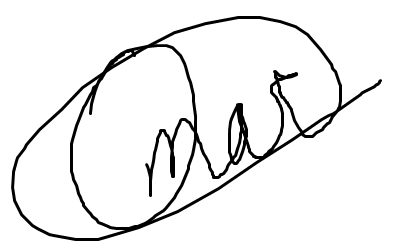
\includegraphics[scale=0.3]{omar-signature.png}\\
	\item \begin{itemize} \end{itemize}
	\item Luka Mahrt-Smith:
	\begin{itemize}
		\item Section 1.3 - Overview
		\item Section 2 - Analysis Class Diagram
	\end{itemize} 
 	
\includegraphics[scale=0.3]{luka_signature.png}\\
	\item Aidan Lao:
	\item \begin{itemize} \end{itemize}
	
	
	
\end{itemize}
% End Section


\end{document}
%------------------------------------------------------------------------------
